\chapter{Método de Desarrollo}

\section{Metodología para la obtención de datos reales}

En adición a la parte técnica, el proyecto contempló bajo una metodología, la obtención de datos reales sobre estafa, puntualmente ejemplos de mensajería fraudulenta que busca explotar a la víctima mediante métodos afines al \textbf{\textit{catfishing}} y la \textbf{\textit{sextorsión}}.

Se llevó a cabo una investigación en foros de internet como Reddit \cite{RedditFlirtu2025}, con el objetivo de encontrar una aplicación de mensajería con reportes frecuentes de estafas.

Los resultados de esta primera fase arrojaron una aplicación candidata por las características difundidas por sus usuarios en el uso de esta plataforma. Se trata de un chat de citas llamado Flirt U, en sentido estricto, un \textbf{\textit{bot de telegram}} el cual se utiliza dentro de dicha plataforma.
\cite{RedditFlirtu2025}
\cite{telegramRisks}

\subsection{Metodología: Perfil señuelo}

Esta tarea involucró al realizar una cuenta señuelo para poder identificar y contactar con posibles estafadores dentro de la aplicación de citas.

El objetivo de esta etapa fue, puntualmente, determinar cuáles eran los patrones clave de cada tipo de estafa: catfishing y \textbf{\textit{sextorsión}}, así como el estilo del lenguaje y la forma de comunicación que suelen emplear los estafadores, por un lado para la generación sintética de datos y, por otro, para la obtención de datos reales.

La \textbf{\textit{recolección de datos}} se remitió exclusivamente a medios de texto, no se contempló imagen.

\subsection{Hallazgos clave de la investigación controlada en Flirtu}

De los atacantes:
* Se encontró que los estafadores, de manera contraintuitiva respecto a parte de los datos sintéticos, suelen pedir con frecuencia realizar videollamadas; efectivamente, se registraron casos en los cuales, del lado del atacante, se visualizaban videos posiblemente falsos con el fin de otorgar confianza.

\subsubsection{Características sobre el catfishing}

\begin{itemize}
    \item Crear historias difíciles para generar empatía en la víctima
    \item Establecer una comunicación que parezca genuina, con el fin de conectar con la víctima y establecer un lazo de confianza que posteriormente puedan explotar para obtener beneficios.
    \item Las solicitudes que efectúan a las víctimas pueden tener diferentes técnicas psicológicas
    \item Solicitar tarjetas de pago, dinero o fotos
    \item Algunos perfiles aprovechaban la conexión emocional para reclutar participantes en grupos de inversión en criptomonedas, cuyas motivaciones no son identificadas en la investigación
    \item Solicitudes constantes para acordar realizar una videollamada de carácter íntimo, mayormente con el objetivo de recabar imágenes privadas con fines de sextorsión y utilizarlas posteriormente en el ejercicio de catfishing con otras víctimas.
    \item Enviar contenido de carácter explícito, en ocasiones coherente con la identidad falsa, con el fin de generar credibilidad.
\end{itemize}

\subsubsection{Características de la sextorsión} 
\begin{itemize}
    \item Solicitan perfil de redes sociales personales con propósitos como:
        \begin{itemize}
            \item Conocer detalles personales de la víctima
            \item Potencialmente acceder a la red de contactos de la persona para después chantajear tras recibir material explícito
        \end{itemize}
    \item Solicitar contenido particularmente explícito, fotografías o videos.
    \item Usar contenido privado de las víctimas para extorsionar bajo la amenaza de publicarlo o enviarlo a cercanos, jefes o parientes, con motivaciones variadas, siendo las principales dinero o más material explícito.
\end{itemize}

\subsection{\textbf{\textit{Recolección}} y \textbf{\textit{etiquetado de datos}}}

Esta etapa de \textbf{\textit{recolección}} de datos implicó la creación de una cuenta en Flirt U, un \textbf{\textit{bot de Telegram}} (destinado a buscar relaciones amorosas, “app de citas”), y establecer contacto con personas que sugería la aplicación. Cabe mencionar que en este proceso se identificó una cantidad de interacción desproporcionada y poco orgánica.

Se estableció un diálogo dentro del mismo grupo que genera el \textbf{\textit{bot de Telegram}}; el mismo bot advierte sobre no llevar las comunicaciones a otro sitio y priorizar establecerlas dentro del grupo creado. En la mayoría de casos se trataba de comunicaciones fraudulentas en las cuales se observaba una transición rápida entre primer contacto y coerción. De igual manera, se solicitaba trasladar las comunicaciones a un chat privado.

Para cada caso se procedió a comunicarse desde el chat privado y seguir un flujo conversacional esperado por el atacante. A lo largo de los diferentes casos se identificaron solicitudes de diversas índoles, denotando los diferentes tipos de motivación relacionados con este fenómeno. De esta manera, se consolidan los hallazgos documentados en la presente investigación.

Posteriormente, tras una muestra de 7 conversaciones, se procedió con la extracción de datos, aprovechando las características de Telegram, el cual permite exportar las conversaciones en formato HTML. Después, se procedió con un proceso de limpieza de datos para almacenar los ejemplos de manera curada, eliminando ruido, dado que en parte de los casos se presentaron errores léxicos y gramaticales.

\section{Generación sintética de data set para refinamiento}

El presente proyecto contempló la \textbf{\textit{recolección de datos}} reales sobre estafas; correspondientemente a los límites y alcances de la investigación, esta \textbf{\textit{recolección}} no fue masiva, por lo que se adoptó una metodología basada en la generación sintética de datos para la construcción del conjunto de datos de refinamiento.
Para conseguir este propósito, se siguieron 8 buenas prácticas para la generación sintética de datos que propone IBM. \cite{SynthDataByIbm} \linebreak \linebreak
Los pasos que se siguieron para generar datos sintéticos: \linebreak
1.- \textbf{\textit{Recolección}} y \textbf{\textit{etiquetado de datos}} reales (mayores detalles en la sección “Metodología: Perfil controlado de observación”).\linebreak
2.- Creación de un prompt basado en la técnica de prompting few shot donde se establecen las características que deben tener los datos así como los ejemplos recolectados.\linebreak
3.- \textbf{\textit{Síntesis de datos}} a partir de modelos largos de lenguaje de gran escala, incluyendo modelos como: Claude Opus 4.6, GPT-5.2 y Gemini 3 Pro.\linebreak
4.- Revisión manual de los ejemplos generados priorizando realismo y diversidad.\linebreak
5.- Construcción de un conjunto de datos de refinamiento a partir de \textbf{\textit{datos sintéticos}} y de un conjunto de datos de pruebas a partir de los datos reales.\linebreak


\subsection{Pruebas de \textbf{\textit{desempeño de clasificación}} en LLMs}

Se contempla el uso de técnicas de \textbf{\textit{prompt engineering}} para maximizar la capacidad de modelos de lenguaje (LLM) en la tarea de clasificación de mensajes sospechosos.

La etapa inicial de esta investigación contempló efectuar un conjunto de pruebas a una colección de modelos largos de lenguaje pertenecientes al actual estado del arte de la inteligencia artificial; se incluyen a continuación:
\linebreak
Qwen3-VL: 4b, Gemma3n: e4b, e2b, Gemma3: 1b, 4b, Gemma2: 2b, Mistral: 7b, Spam-Detect: latest, Qwen3: 8b, 4b, 1.7b, 0.6b, EmotionAI: latest, SmallThinker: 3b, Qwen2.5: 7b, 3b, 1.5b, 0.5b, Phi4-mini: 3.8b, Phi4-mini-reasoning: 3.8b, Llama-Guard3: 8b, 1b, TinyDolphin: 1.1b, Llama3: 8b, Llama3.2: 3b, 1b, Llama3.1: 8b, Llama-3-Refueled: Q4\_K\_M, Opus-v1.2: Q4\_K\_M, Granite3.2: 8b, 2b, Granite3.3: 8b, 2b, Dolphin3: 8b, DeepSeek-R1: 8b, 1.5b, DeepCoder: 1.5b, Cogito: 3b, 8b, ALIENTELLIGENCE/emotionalintelligenceanalysis:latest, ahmadwaqar/smolvlm2-500m-video:fp16, ahmadwaqar/smolvlm2-500m-video:q8, llama-pro:instruct, granite3.2-vision:2b, minicpm-v:8b, bakllava:7b, qwen2.5vl:3b, qwen2.5vl:7b, qwen3-vl:2b, qwen3-vl:4b, qwen3-vl:8b, llava:7b, codegemma:2b, codegemma:7b, starcoder2:3b, starcoder2:7b, wizard-vicuna-uncensored:7b, openthinker:7b, granite3.1-moe:1b, granite3.1-moe:3b, smollm:135m, smollm2:135m, smollm:360m, smollm2:360m, falcon3:1b, smollm:1.7b, smollm2:1.7b, tinyllama:1.1b, phi:2.7b, orca-mini:3b, falcon3:3b, stablelm2:1.6b, exaone-deep:2.4b, exaone-deep:7.8b, neural-chat:7b, falcon:7b, dolphin-llama3:8b, zephyr:7b, openchat:7b, orca-mini:7b, falcon3:7b, olmo2:7b, olmo-3:7b, phi3:3.8b, ministral-3:3b, ministral-3:8b.

El propósito de estas pruebas es determinar el conjunto de modelos con mayor \textbf{\textit{ponderación}} mediante la comparación del desempeño de esta selección de modelos en la clasificación de catfishing y \textbf{\textit{sextorsión}}, así como métricas relacionadas con el tamaño de los modelos (número de \textbf{\textit{parámetros}}) y tiempo promedio por predicción. Para las pruebas, se contempló refinamiento mediante técnicas de prompting bajo los enfoques zero-shot y few-shot, para determinar el modelo que se empleará en la aplicación de mensajería.

La metodología empleada para llevar a cabo este conjunto de pruebas contempló el desarrollo de un código en Python donde se programó la lógica para la ejecución de los modelos, evaluación a través de métricas y almacenamiento de resultados. La presentación de los resultados se realiza en la sección “Pruebas y resultados”.

\begin{figure}[H]
    \centering
    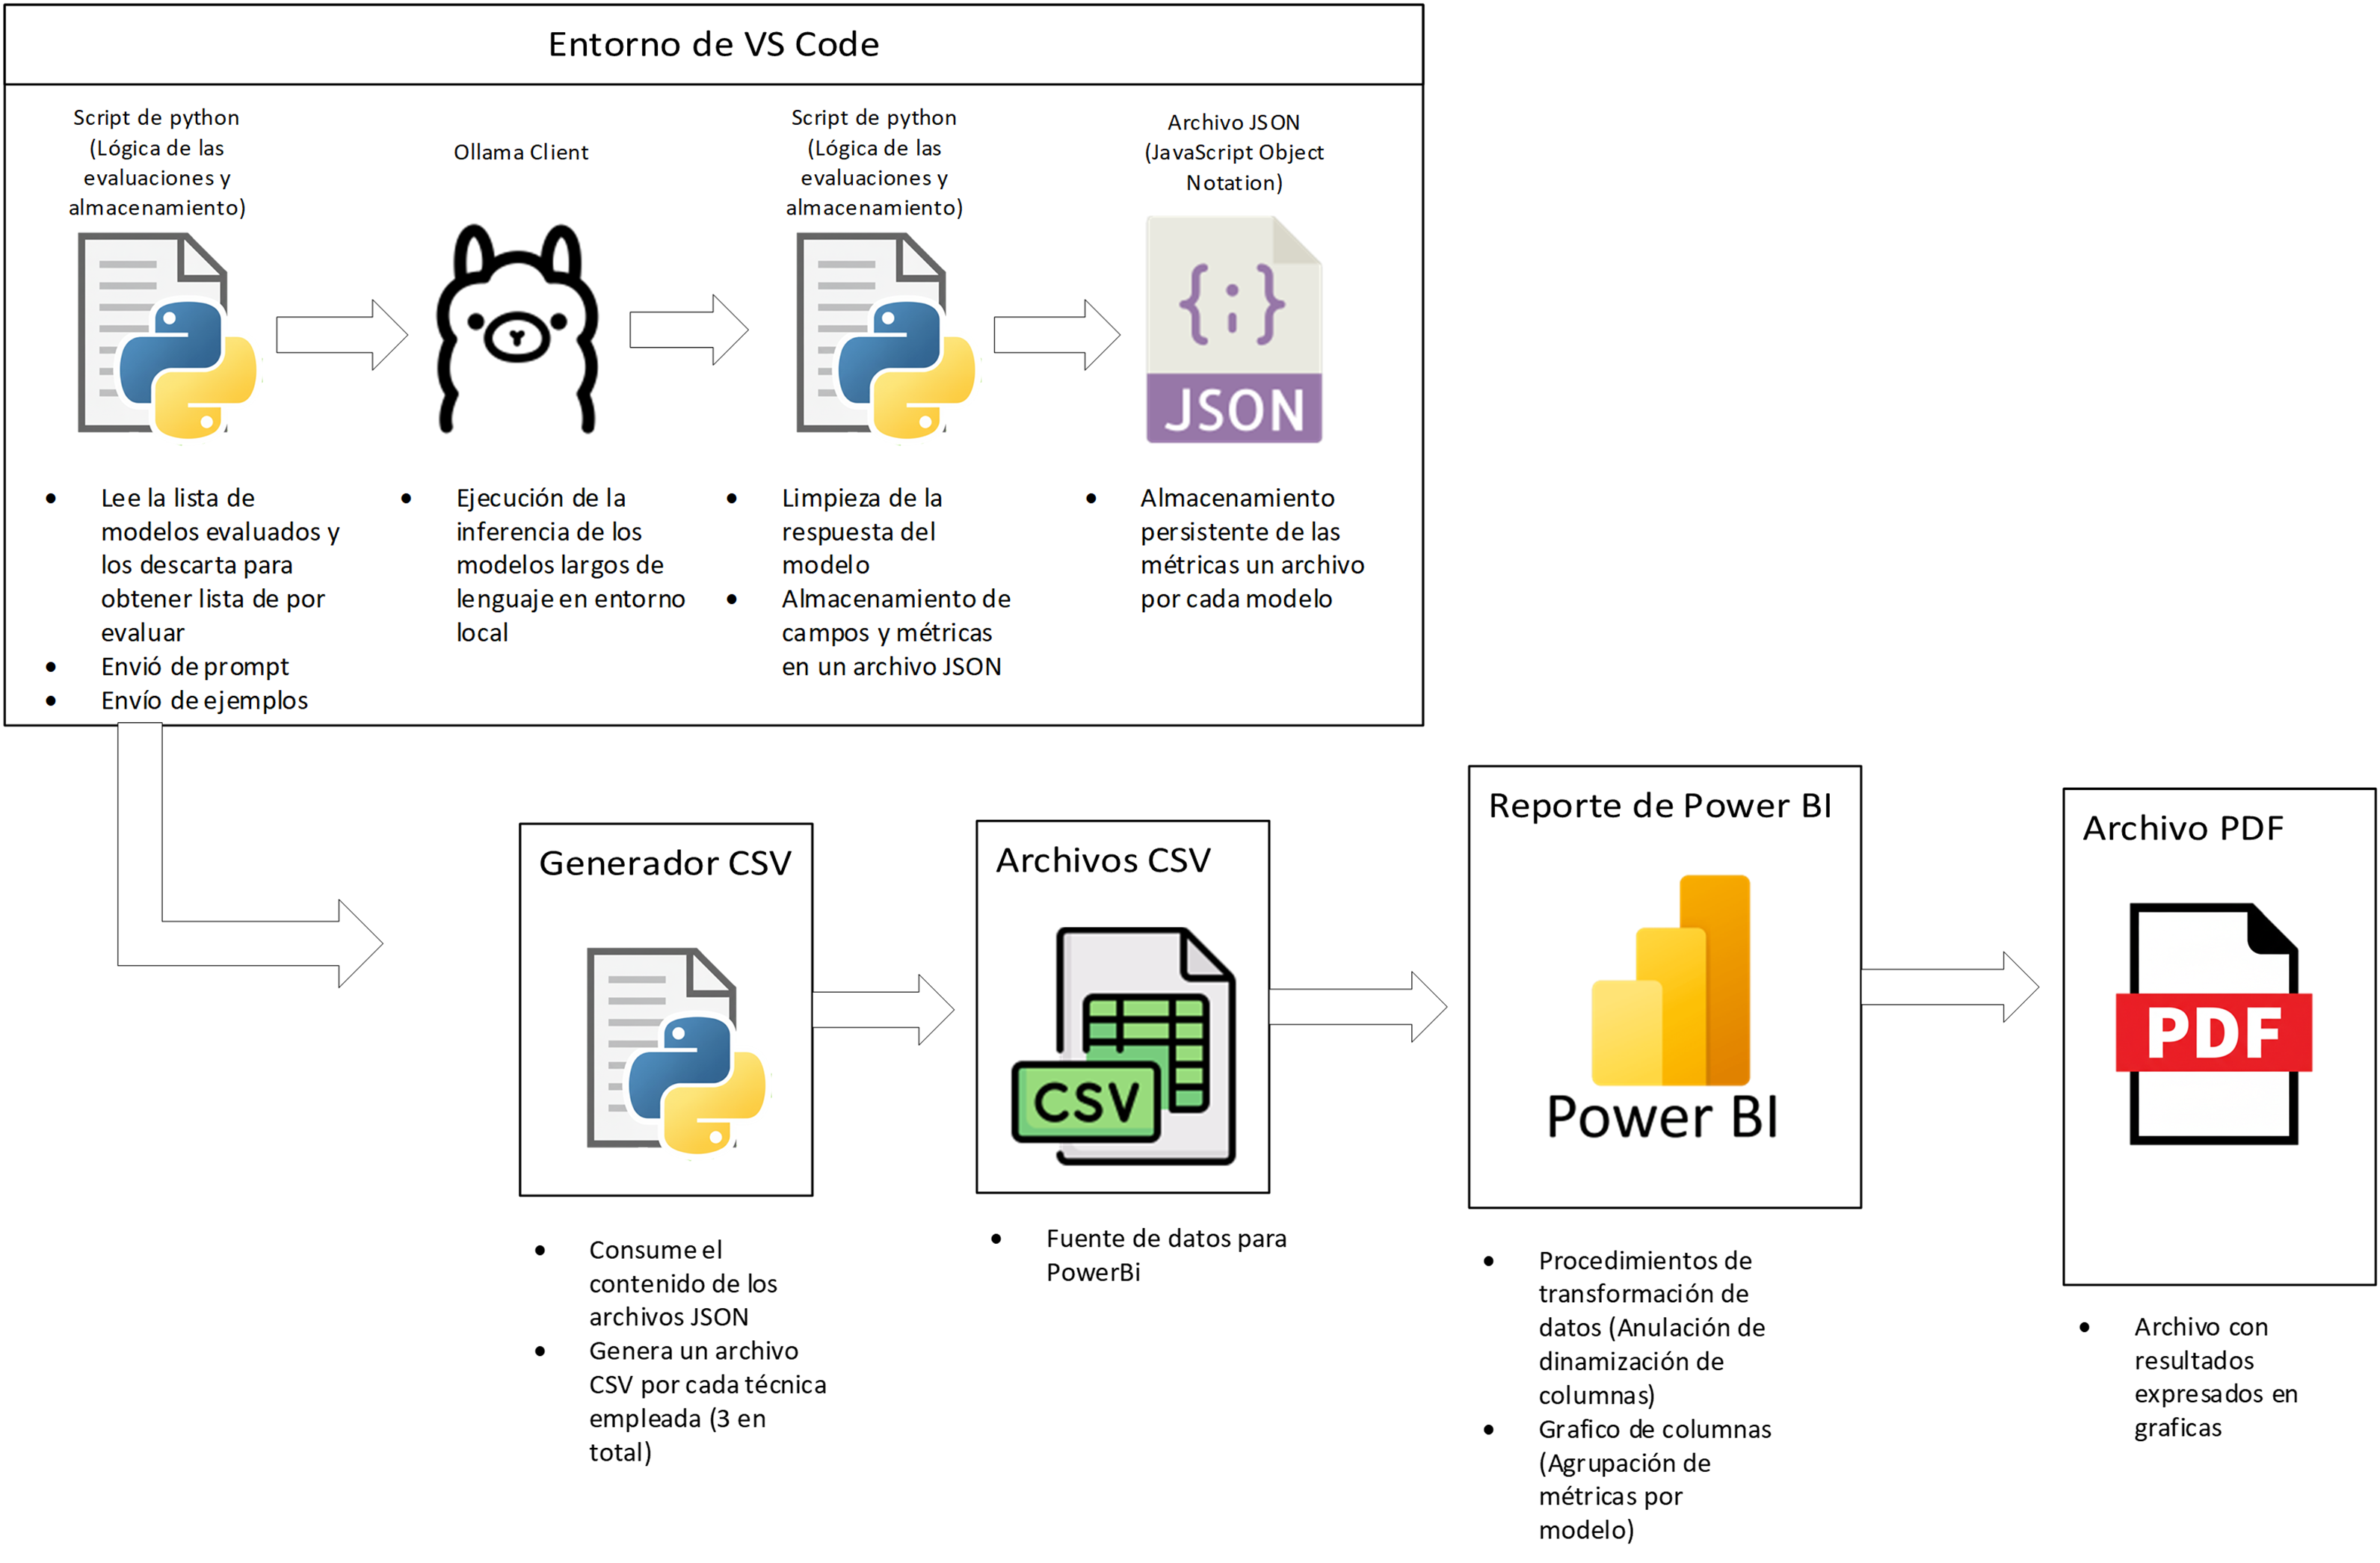
\includegraphics[width=0.9\linewidth]{imagenes/pruebas/diagEnvTest.png}
    \caption{Diagrama arquitectónico del entorno de pruebas de clasificación para evaluación de LLMs}
    \label{fig:diagrama-entorno-pruebas}
\end{figure}

\textbf{Dirigirse a los anexos 7.3 y 7.4 para observar el prompt de refinamiento empleado en las pruebas reportadas asi como los modulos mas relevantes del entorno de pruebas escrito en python en el orden respectivo.}

\section{Arquitectura de solución}

\subsection{Arquitectura general del sistema (explicación)}

\begin{figure}[H]
    \centering
    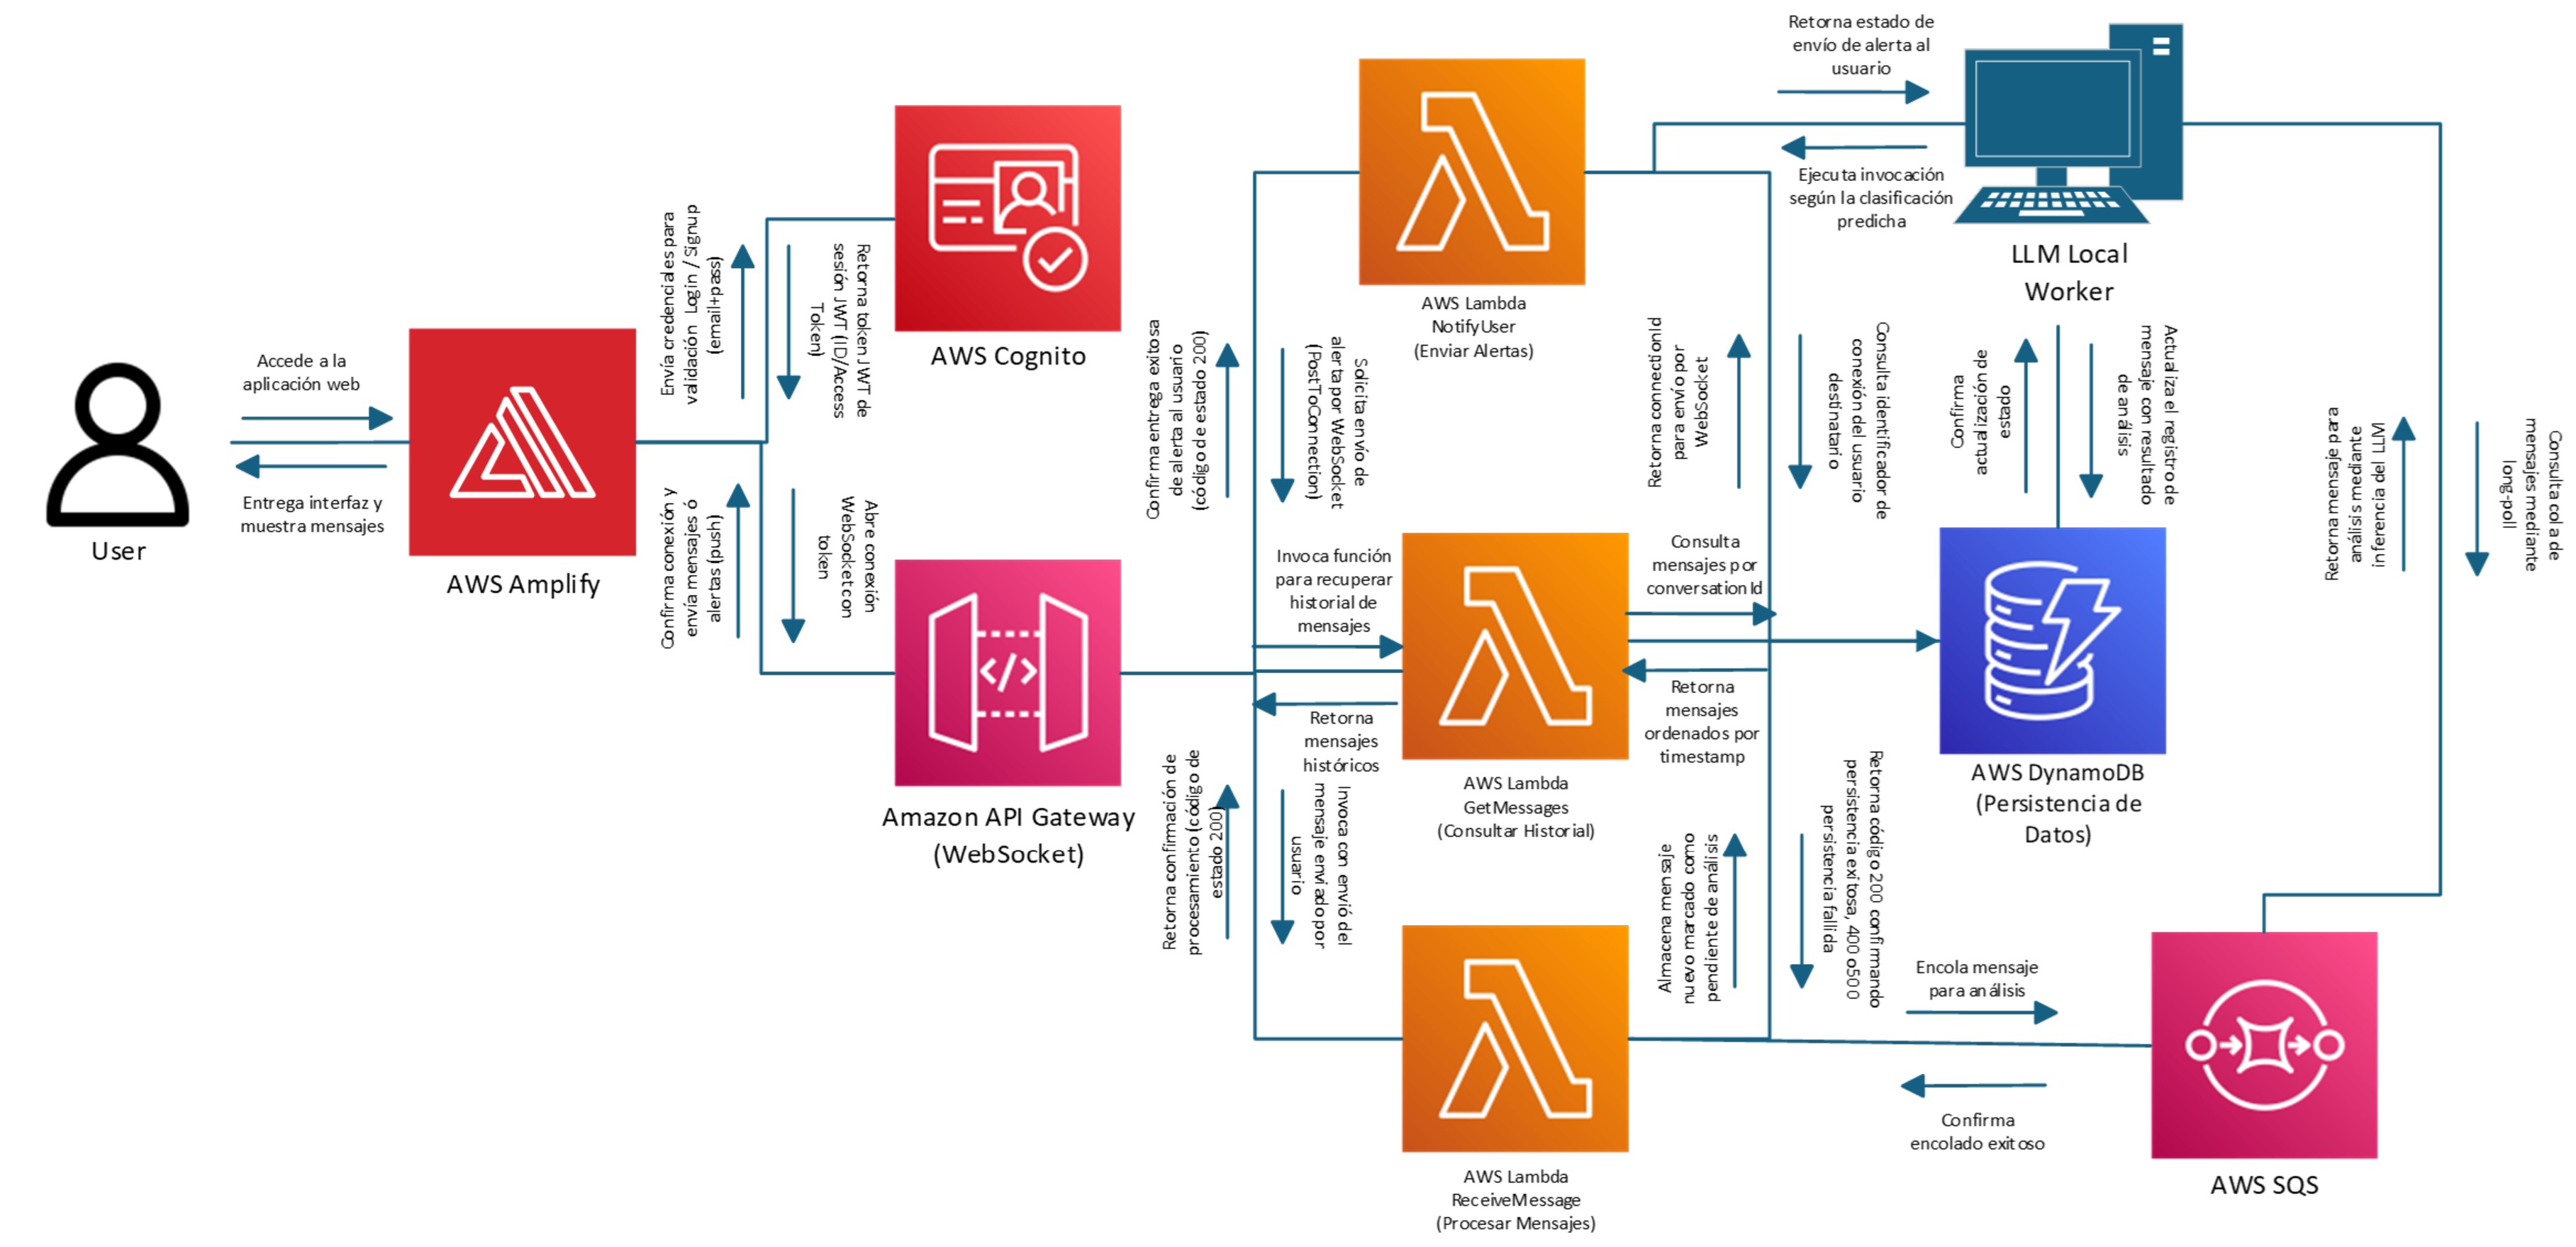
\includegraphics[width=0.9\linewidth]{imagenes/desarrollo/propuestaSolucion/diagramaArquitectonico.pdf}
    \caption{Diagrama arquitectónico: Arquitectura de Servicios AWS de la Aplicación de mensajería}
    \label{fig:diagrama-arquitectonico}
\end{figure}

Se propone una solución híbrida contemplando cómputo en la nube mediante los servicios administrados de AWS y procesamiento local para la ejecución de la \textbf{\textit{inferencia}} del modelo a largo de lenguaje para el análisis de contenido.

El sistema está diseñado para detectar técnicas de \textbf{\textit{sextorsión}} y \textbf{\textit{catfishing}} en conversaciones de chat, alertando a los usuarios de manera preventiva cuando se identifiquen patrones de riesgo, mientras se cuenta con persistencia de datos y requerimientos funcionales de un sistema de mensajería.

\subsection{Descripción de la arquitectura por servicio de Amazon web services}

La arquitectura es una solución híbrida nube-local diseñada para implementar un sistema de \textbf{\textit{mensajería instantánea}} con características de inteligencia artificial para la detección de estafas en modalidad de \textbf{\textit{catfishing}} y/o \textbf{\textit{sextorsión}}. Esta arquitectura se fundamenta en la escalabilidad y confiabilidad de los servicios del \textbf{\textit{ecosistema}} AWS y en el procesamiento local de la \textbf{\textit{inferencia}} de modelos largos de lenguaje (LLM) como clasificadores. El presente diseño está contemplado para la detección de mensajería catalogada como \textbf{\textit{catfishing}} o \textbf{\textit{sextorsión}} dentro de conversaciones de chat, con el objetivo de alertar de manera preventiva a usuarios potencialmente víctimas cuando el sistema identifique patrones de riesgo; todo integrado en un sistema de mensajería con persistencia de datos y gestión de usuarios.

\subsubsection{1. AWS AMPLIFY HOSTING (\textbf{\textit{Frontend}})}

AWS Amplify es un servicio de AWS empleado para alojar y servir el front end de la aplicación web, del lado del cliente. Este servicio permite desplegar aplicaciones desde repositorios Git.

Su funcion es servir los archivos estaticos del front end que incluyen html, css y JavaScript, es compatible con el certificado \textbf{\textit{SSL/TLS}} por lo que sirve conexiones seguras a traves de \textbf{\textit{HTTPS}}. 

Su uso dentro del presente proyecto radica en simplificar la complejidad del desarrollo en relacion a la configuracion de servidores web y aspectos relacionados a la gestion certificados SSL. De entre las caracteristicas por las que se contempla dentro del proyecto es su generosa capa gratuita que incluye 15GB de almacenamiento en la infraestructura de AWS asi como la compatibilidad con los demas servicios de la capa gratuita de AWS. 

\subsubsection{2. AMAZON COGNITO USER POOL (Autenticación)}

Amazon Cognito User Pool es un servicio de AWS orientado a la autenticación de usuarios, maneja funcionalidades desde el registro hasta la recuperación de credenciales.

Su funcion es servir como un sistema de autenticacion estable, gracias a que esta basado en estandares como \textbf{\textit{OAuth 2.0}} y OpenID Connect. mediante la generacion de \textbf{\textit{JWT (Json Web Tokens)}} permiten validar las credenciales de usuarios, estos son empleados para autorizar peticiones hacia \textbf{\textit{API}} Gateway y otros servicios dentro del \textbf{\textit{ecosistema}} AWS. 

Su uso dentro del presente proyecto es requerido para implementar un sistema de autentificacion seguro, lo cual es un proyecto de amplia madurez y complejidad en si mismo, ademas de ser propenso a vulnerabilidades. Cognito provee de una solucion robusta que brinda hash de contraseñas bcrypt, protección contra ataques de fuerza bruta, verificación de email, y cumplimiento con estándares de seguridad.

\subsubsection{3. API GATEWAY \textbf{\textit{WebSocket}} \textbf{\textit{API}} (Comunicación en \textbf{\textit{tiempo síncrono}}.)}

\textbf{\textit{API}} Gateway con soporte \textbf{\textit{WebSocket}} es el servicio dentro de AWS que establece conexiones bidireccionales entre clientes y \textbf{\textit{backend}}, permitiendo la comunicación en \textbf{\textit{tiempo síncrono}}.

Su función es servir como medio de enlace con cada uno de los clientes que consumen la aplicación; este asigna un connectionId a cada sesión. Entre otras cosas, gestiona el envío de mensajes dentro de la aplicación y es responsable del enrutamiento hacia la función Lambda, dependiendo del flujo de datos, en casos como "enviar mensaje", "obtener historial" y "recibir mensaje". También será empleado por el requerimiento de envío de mensajes desde el backend hasta los clientes, para gestionar el alertamiento oportuno mediante mensajes que lleguen a la interfaz de usuario.

Su uso es requerido dentro del proyecto en alineación con el objetivo del diseño de un sistema de mensajería similar a los medios de redes sociales actuales como WhatsApp o Telegram. En estos casos se emplea una comunicación bidireccional de \textbf{\textit{tiempo síncrono}}; esto se logrará mediante una \textbf{\textit{API}} de tipo \textbf{\textit{WebSocket}}, la cual mantiene una conexión \textbf{\textit{TCP}} persistente que permite comunicación bidireccional. El servicio de AWS tiene incorporadas características propias de los sistemas de comunicación, como el manejo de errores y la reconexión; en adición, posee integración con AWS Lambda.

\subsubsection{4. AWS LAMBDA - ReceiveMessage (Procesamiento de Mensajes Entrantes)}

Las funciones Lambda de AWS son su alternativa a las denominadas funciones serverless, caracterizadas por no requerir \textbf{\textit{aprovisionamiento}} de alli la descripcion serverless equivalente a "sin servidor".

La función de este servicio se concentra en el procesamiento de la lógica de programación definida. Algunas de sus tareas incluyen almacenar los mensajes recibidos en la base de datos de AWS DynamoDB, encolar el mensaje empleando el servicio AWS SQS para su análisis posterior por parte del worker local (el modelo gestionado en máquina local) y reenviar el mensaje a su destinatario a través del servicio AWS API Gateway WebSocket.

Su uso en el proyecto es fundamental para la implementación de la lógica del \textbf{\textit{backend}}. Son requeridas, de igual manera, para la gestión de la lógica de desacoplamiento asíncrono: gracias a la encolación desde SQS, se consigue que el procesamiento de la \textbf{\textit{inferencia}} del LLM en el worker local sea independiente del flujo de datos principal perteneciente a la funcionalidad del sistema de mensajería. De esta manera, la ejecución del modelo no retrasa el envío y recepción de mensajes. En adición, una de las principales características de las funciones Lambda es la facturación, la cual puede ser en función de las ejecuciones, lo que ahorra costos de \textbf{\textit{aprovisionamiento}} desperdiciado, pues solo se cobra por las ejecuciones realizadas.

\subsubsection{5. AWS LAMBDA - GetMessages (Recuperación de Historial)}

Se define la función de nombre "GetMessages" dentro del diseño; esta llevará la lógica encargada de recuperar el historial de conversaciones para cada usuario.

Su función en la arquitectura propuesta es consultar dentro de DynamoDB los mensajes, así como metadatos de estos, por ejemplo, el estado de su análisis y si fue reportada alguna alerta sobre los mismos.

Dentro de las caracteristicas que consolidan la necesidad de delegar la funconalidad de recuperación de historial a esta funcion es la paginacion dentro de conversaciones largas, ademas de contar con un diseño modular segmentado por funcionalidad.

\subsubsection{6. AWS LAMBDA - NotifyUser (Sistema de Alertas)}

Esta funcion lambda es la encargada de notificar al front end del cliete cuanto el worker identifica contenido relacionado a catfishing y sextorsion  

En terminos de su funcionalidad, esta funcion es invocada por el worker cuando el mismo arroja un resultado de prediccion sobre catfishing o sectorsion, la funcion hace consultas a DynamoDB para obtener el id de coneccion del usuario para identificar al usuario que debe recibir el alertamiento, la notificacion de alerta es enviada a traves del servicio de API Gateway de WebSocket directo al cliente conectado

Esta funcion es responsable de una de las partes mas criticas del sistema responsable de alertar al usuario para lograr la prevencion de la estafa, ademas consolidar esta funcion permite obtener un modulo que posteriormente pueda ser ampliado en funcionalidades y gestionar aspectos como los son, el escalamiento de notificaciones en funcion del riezgo detectado o registro de notificaiones para auditorias.

\subsubsection{7. AMAZON DYNAMODB (Persistencia de Datos)}

El serviccio de DynamoDB se consolida como una base de datos \textbf{\textit{NoSQL}} perteneciente al \textbf{\textit{ecosistema}} AWS, es el servicio encargado de almacenar los datos del sistema como mensajes y metadatos de conversaciones.

Dentro de la tabla de ChatMessages se emplea conversationId como clave de particion "PK" y timestanmp como clave de ordenamiento "SK", de esta manera los mensajes se presentan en orden cronologico, algunos campos notables son: messageId, senderId, receiverId, content, status, analysisResult, connectionId, entre otros.

DynamoDB es requerido en el presente proyecto por caracteristicas como 
tener una \textbf{\textit{latencia}} de milisegundos, permitir el \textbf{\textit{escalamiento}} automatico y la disponibilidad en adicion con no requerir \textbf{\textit{aprovisionamiento}}. Dentro del contexto de un sistema de mensajeria es totalmente necesario tanto por la persistencia de los datos como por todas las caracteriscas mencionadas las cuales son necesarias para tener consultas de mensajes rapidas asi como la posibilidad para soportar picos de escitura conforme al trafico.

\subsubsection{8. AMAZON SQS - MessageAnalysisQueue (Cola de Análisis)}

Amazon "SQS Simple Queue Service" es el servicio que tiene como tarea el encolamiento de mensajes, es un \textbf{\textit{buffer de memoria}} entre el sistema de mensajeria y el Worker local que ejecuta el LLM mediante ollama.

El flujo de los datos respecto a este servicio inicia despues de hacer sido almacenado un mensaje en DynamoDB, esta cola se configurara con long-polling de 20 segundos (periodo de consulta por parte del worker hacia la cola en SQS), posteriormente el worker procesa cada mensajes mediante el LLM, y los elimina de la cola tras actualizar el estatus en el registro de DynamoDB.

La necesidad de SQS dentro del proyecto en buena medida se refiere a los mecanismos para tolerancia a fallos considerando la arquitectura hibrica cloud - local, se requiere para manejar casos como tener la computadora local apagada o sin conexión, esto permite garantizar que ningún mensaje quede sin analizar. 

\subsubsection{9. AMAZON SQS - Dead Letter Queue (Gestión de Fallos)}

Esta es una cola secundaria conocida como DLQ esta recibe los mensajes en los que no se concreto el analisis después de múltiples intentos.

Cuando un mensaje falle un numero de veces consecutivas SQS movera el mensaje a DQL estos mensajes quedaran disponibles para inspección manual o reprocesamiento.

Es requerida puesto que de no emplearse los mensajes que no pudieron ser analizados bloquearian la cola principal SQS en un ciclo infinito de reintentos lo cual imposibilitaria continuar con los demas mensajes, adicionalmente las DLQ pueden permitir la identificacion de problemas sistematicos en funcion de patrones problematicos en los mensajes. 

\subsubsection{10. WORKER LOCAL + OLLAMA LLM (Análisis de Contenido)}

Lo que en esta seccion se ha referenciado como "Worker" se refiere concretametne a una aplicacion de Python que se ejecuta en la computadora local y el cual gestiona las llamadas a los modelos mediante el cliente de Ollama al igual que la comunicacion con los demas servicios dentro de la infraestructura de AWS.

Este codigo ejecuta en ciclos lo siguiente: 1.- SQS para obtención de mensajes pendientes de analisis, 2.- Enviar el contenido del mensaje al modelo que corre local mediante el cliente ollama, 3.- Recepcion de la etiqueta predicha por el modelo, 4.- Actualiza el estado de analisis en los registros de la base de datos en DynamoDB, 5.- invoca a la función Lambda "NotifyUser" para alertar al usuario en caso de haber recivido prediccion de estafa, y 6.- Eliminar el mensaje de la cola SQS después de confirmar todas las operaciones.

Este componente o servicio local es necesario y forma parte de la parte mas relevante del proyecto encargado de la ejecucion de la \textbf{\textit{inferencia}} del modelo asi como de las operaciones pertinentes para clasificar los mensajes, ademas el que se implemente de manera local permite reduccion de costos en contraste con la alternativa en cloud que involucra pagar por \textbf{\textit{inferencia}} en los servicios de AWS "SageMaker" o "Bedrock". De esta manera se ajusta a los limites establecidos en el presente proyecto  y permite emplear una coleccion basta de modelos los mismos que fueron evaluardos en la seccion de pruebas. 

Se contemplo emplear modelos con \textbf{\textit{escalas}} de entre 0.25 billones de \textbf{\textit{parámetros}} hasta 8 billones de \textbf{\textit{parámetros}} dentro de hardware local con las siguientes caracteristicas: (CPU Intel(R) Core(TM) i7-4770 4ª generación  basada en la arquitectura Haswell Frecuencia base de 3.40GHz, GPU Nvidia GeForce GTX 1060 6GB \textbf{\textit{VRAM}}, 16GB Ram del sistema con frecuencia de 1600 MHz, Almacenamiento persistente ADATA HD720 SCSI 1.8 terabytes).

\section{Entorno de desarrollo local}

En conformidad con los limites y alcances del presente proyecto, la propuesta de solución fue desarrollada en un ambiente enteramente local. Esta delimitacion implico emplear una emulación local los servicios del ecosistema AWS definidos en la seccion anterior, mediante las tecnologias docker y local-stack, un plugin perteneciente al proyecto serverless framework.

A continuación se adjuntan 2 diagramas sobre el entorno de producción definido en el desarrollo del sistema, el mismo emplea docker para encapsular la emulacion de los servicios AWS dentro de un contenedor independiante al sistema operativo anfitrión.

\begin{figure}[H]
    \centering
    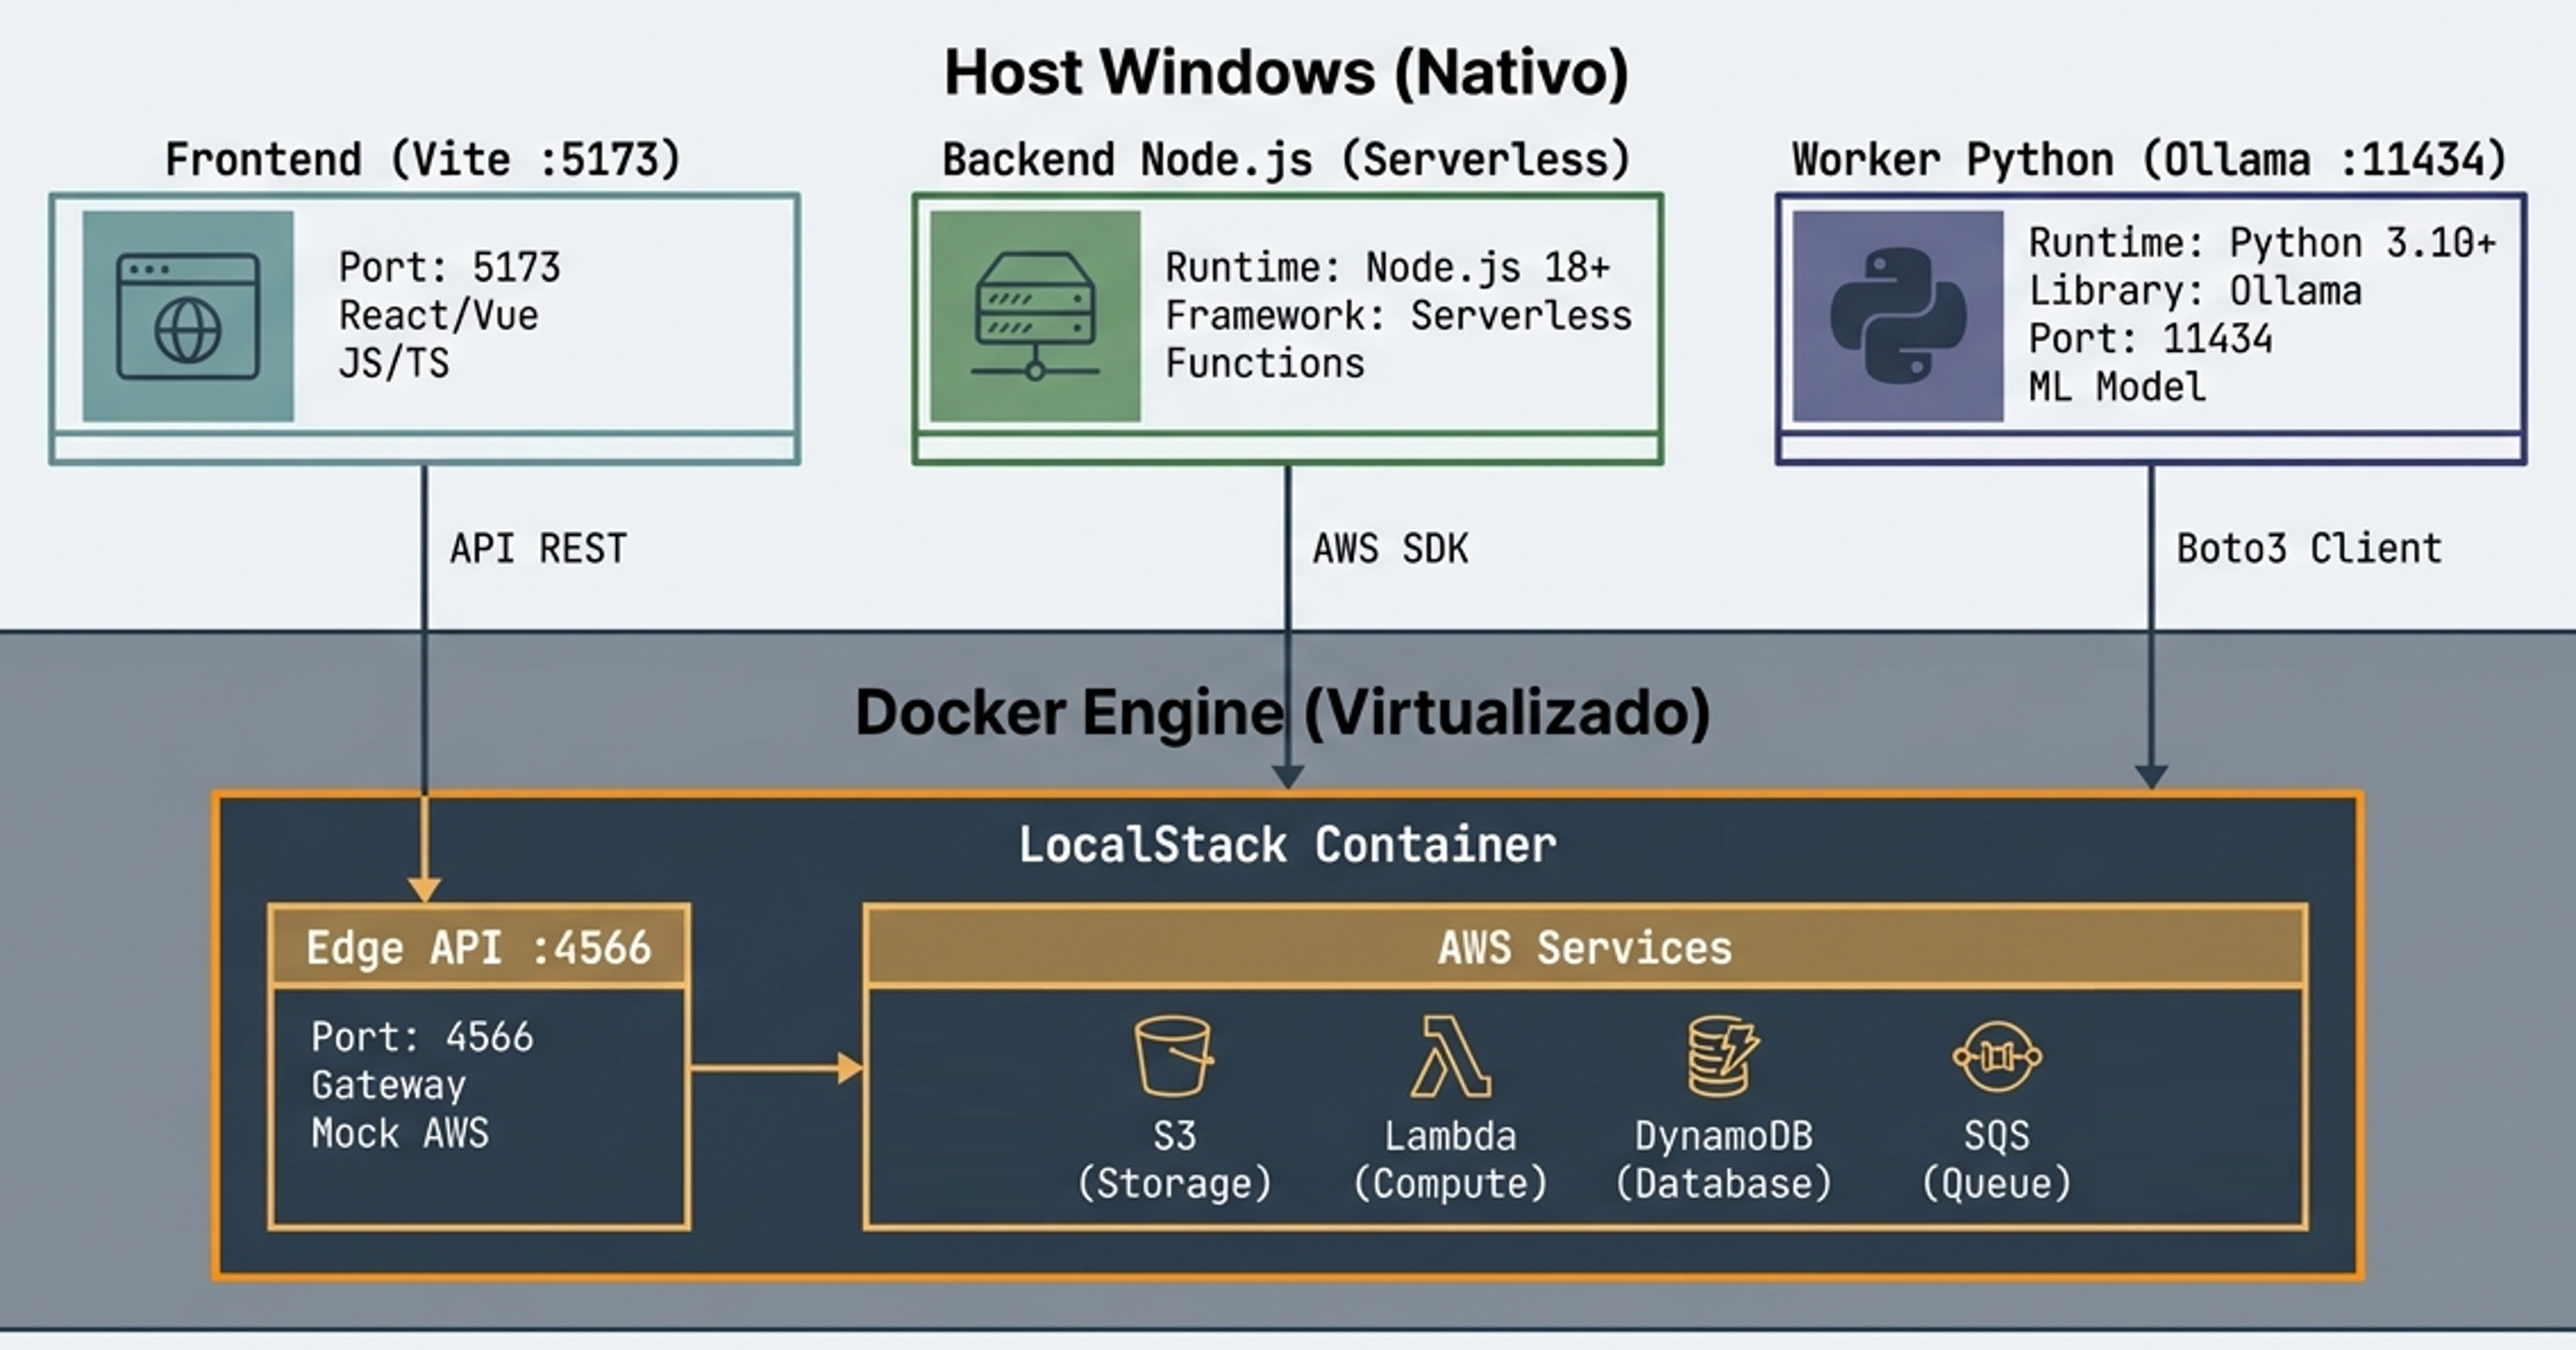
\includegraphics[width=0.9\linewidth]{imagenes/desarrollo/diagramaComponentes2.png}
    \caption{Diagrama de topología lógica: Entorno de desarrollo local, Aplicación de mensajería con analisis conversacional mediante llms. \textit{Diagrama creado mediante notebookLM a partir de fuentes propias}}
\end{figure}

\begin{figure}[H]
    \centering
    
\includegraphics[width=0.9\linewidth]{\detokenize{imagenes/desarrollo/diagramaFlujoDatos.png}}
    \caption{Diagrama de flujo de datos: Entorno de desarrollo local, Aplicación de mensajería con analisis conversacional mediante llms. \textit{Diagrama creado mediante notebookLM a partir de fuentes propias}}
\end{figure}

\section{Vistas de la aplicacion}

En esta seccion se muestran las vistas de la aplicación de mensajería con la arquitectura anteriormente descrita.

\subsubsection{Vistas del LogIn (Inicio de sesión)}

Estas capturas muestran la interfaz de inicio de sesion, el caso 2 muestra la interfaz cuando se intenta acceder con credenciales no registradas en la base de datos de dynamodb

\begin{figure}[H]
    \centering
    
\includegraphics[width=0.9\linewidth]{\detokenize{imagenes/mockUps/Log In.png}}
    \caption{Vista de inicio de sesión}
\end{figure}

\begin{figure}[H]
    \centering
    
\includegraphics[width=0.9\linewidth]{\detokenize{imagenes/mockUps/Log In false.png}}
    \caption{Inicio de sesion con error de credenciales}
\end{figure}

\subsubsection{Vistas del registro}

Aqui se muestra el registro de un usuario, se solicita un nombre de usuario y contraseña.

\begin{figure}[H]
    \centering
    
\includegraphics[width=0.9\linewidth]{\detokenize{imagenes/mockUps/Registro.png}}
    \caption{Formulario de registro}
\end{figure}

\begin{figure}[H]
    \centering
    
\includegraphics[width=0.9\linewidth]{\detokenize{imagenes/mockUps/Registro 2.png}}
    \caption{Procesamiento del registro}
\end{figure}

\subsubsection{Vistas de chat y agregar contacto}

A continuación se observa la ventana de chats que se muestra tras haberse loggeado efectivamente con credenciales validas en el sistema

\begin{figure}[H]
    \centering
    
\includegraphics[width=0.9\linewidth]{\detokenize{imagenes/mockUps/Vista de chat vacio.png}}
    \caption{Vista de chat vacío (usuario sin conversaciones activas)}
\end{figure}

posteriormente tras ingresar a la aplicacion, se puede contactar con otro usuario registrado en la base de datos, para esto hay que dar click en el boton con el signo de + y posteriormente se desplegara este recuadro, el mismo validara la existencia del usuario en el sistema y de ser procedente creara un nuevo chat con el usuario.  

\begin{figure}[H]
    \centering
    
\includegraphics[width=0.9\linewidth]{\detokenize{imagenes/mockUps/Vista de crear contacto.png}}
    \caption{Vista de añadir nuevo contacto}
\end{figure}

Esta es la vista de la ventana cuando se ingresa un usuario que no ha sido registrado.

\begin{figure}[H]
    \centering
    
\includegraphics[width=0.9\linewidth]{\detokenize{imagenes/mockUps/Vista de crear contacto cuando detecta un usuario no registrado.png}}
    \caption{Vista de añadir nuevo contacto con error por usuario no registrado en base de datos}
\end{figure}

Tras buscar algun usuario en la ventana anterior y haber encontrado una coincidencia, el sistema genera un nuevo chat listo para interactuar.  

\begin{figure}[H]
    \centering
    
\includegraphics[width=0.9\linewidth]{\detokenize{imagenes/mockUps/Vista de crear contacto procedente sin chats activos.png}}
    \caption{Vista de chat nuevo sin mensajes}
\end{figure}

Una vez que se ha iniciado una conversacion, el sistema enviara cada mensaje a su analisis mediante el worker de python que ejecuta la inferencia del modelo a traves del cliente de Ollama y en caso de clasificar dicho mensaje como catfishing o sextorsión se mostrará una vista como la siguiente. 

\begin{figure}[H]
    \centering
    
\includegraphics[width=0.9\linewidth]{\detokenize{imagenes/mockUps/notificacionSextorsion.png}}
    \caption{Vista de chat con notificacion de alerta por sextorsión}
\end{figure}

\subsection{Conclusión sobre la arquitectura}

La presente solucion se establece dentro de los servicios que oferta AWS en su capa gratuita, se consolida como un diseño funcional con caracteristicas modulares que permiten un mantenimiento gestionable a futuro, adicionalmente el uso de los diferentes servicios descritos le otorgan al sistema mecanismos de tolerancia a fallos que permiten su funcionamiento, incluso cuando determinados componentes de software dejen de operar.
